% !TEX program = pdflatex
\documentclass{article}

\usepackage{PRIMEarxiv}
\usepackage[utf8]{inputenc}
\usepackage[T1]{fontenc}
\usepackage{hyperref}
\usepackage{url}
\usepackage{booktabs}
\usepackage{amsfonts}
\usepackage{nicefrac}
\usepackage{microtype}
\usepackage{fancyhdr}
\usepackage{graphicx}
\usepackage{enumitem}
\graphicspath{{./}{plots/}{ablation_study/reports/}}

% Header
\pagestyle{fancy}
\thispagestyle{empty}
\rhead{ \textit{ }}
\fancyhead[LO]{Antimicrobial Activity Prediction}

% Title
\title{Peptide--Bacterium Antimicrobial Activity Prediction\\Model, Dataset, and Evaluation Report}

\author{Yann Baglin\-Bunod \\
UC San Diego \\
\texttt{ybaglinbunod@ucsd.edu}}

\begin{document}
\maketitle

\begin{abstract}
We present a dual\-sequence predictor of antimicrobial activity that takes a short bacterial DNA segment and a peptide amino acid sequence as inputs and outputs a binary probability of killing. We describe dataset construction, a Claude\-generated baseline refined into a robust training/evaluation pipeline, and a multi\-seed 70/15/15 split ablation study (ROC/PR, calibration, threshold sweeps). We report accuracy/ROC\-AUC (mean~$\pm$~std) across seeds and release artifacts for reproducibility.
\end{abstract}

\keywords{Antimicrobial peptides, sequence modeling, evaluation, ROC\-AUC, ablation}

\section{Introduction / Background}
\begin{itemize}[leftmargin=*,nosep]
  \item \textbf{Context}: Predict whether a peptide kills a bacterium from sequence inputs.
  \item \textbf{Original direction}: Prompted reasoning models (PRMs), BrowseComp, DreamPRM. Scope shifted per supervisor guidance to a concrete ML task.
  \item \textbf{Supervisor guidance}: Prof. Xie suggested pivoting from PRM to a peptide--bacteria prediction system to test Claude\-generated code in a real pipeline.
\end{itemize}

\section{Objectives}
\begin{itemize}[leftmargin=*,nosep]
  \item Build a working model that predicts peptide lethality given peptide and bacterial DNA.
  \item Subtasks: dataset creation/integration, model implementation, rigorous testing of Claude\-generated code.
  \item Constraints: no single ready\-made dataset; multiple sources must be cleaned/merged into training format.
\end{itemize}

\section{Dataset Development}
\begin{itemize}[leftmargin=*,nosep]
  \item \textbf{Sources}: Materials provided (e.g., target\_organism folder, activity spreadsheets, PubMed abstracts), general AMP databases (e.g., DRAMP), plus a consolidated JSON (\texttt{train\_sequence.json}) when available.
  \item \textbf{Challenges}: Fragmentation, schema inconsistency, missing per\-organism labels; required harmonization.
  \item \textbf{Processing}: Cleaning, normalization, mapping to a unified schema with fields: \texttt{dna\_sequence}, \texttt{protein\_sequence}, \texttt{antimicrobial\_activity}~(0/1). Resulting CSVs are consumed directly by the trainer.
  \item \textbf{Notes}: README descriptions and external database references (e.g., DRAMP) guided integration.
\end{itemize}

\section{Methods / Modeling}
\begin{itemize}[leftmargin=*,nosep]
  \item \textbf{Baseline}: Claude\-generated PyTorch model refined into a stable script (\texttt{antimicrobial\_predictor.py}).
  \item \textbf{Architecture}: Two branches: DNA (Embedding\,$\rightarrow$\,CNN\,$\rightarrow$\,AdaptiveMaxPool) and peptide (Embedding\,$\rightarrow$\,2\-layer BiLSTM\,$\rightarrow$\,8\-head self\-attention\,$\rightarrow$\,masked global average pool). Features are concatenated and fed to an MLP classifier with dropout and sigmoid.
  \item \textbf{Preprocessing}: Integer tokenization; fixed lengths (DNA~50 nt, peptide~100 aa). Length stats: see plots in \texttt{plots/}.
  \item \textbf{Training}: Adam (lr 1e\-3), BCE loss, weight decay 1e\-5, gradient clipping, ReduceLROnPlateau, early stopping. Best model by validation accuracy is versioned; per\-epoch checkpoints saved under \texttt{ablation\_study/runs/}.
\end{itemize}

\section{Results / Preliminary Findings}
\begin{itemize}[leftmargin=*,nosep]
  \item \textbf{Initial validation}: Strong val accuracy and ROC\-AUC on in\-split validation.
  \item \textbf{Claude limitations}: When no data were available, Claude proposed synthetic placeholders; these were replaced by curated CSVs to avoid misleading results.
  \item \textbf{Diagnostics}: Learning curves and sample predictions verified stable training; see \texttt{plots/training\_history.png} and \texttt{plots/model\_overview.png}.
\end{itemize}

\section{Ablation Study and Robust Evaluation}
\textbf{Protocol}: 70/15/15 train/val/test split; 5 random seeds; report test accuracy and ROC\-AUC (mean~$\pm$~std). For each seed, we generate ROC/PR curves, calibration plots, threshold sweeps, confusion matrices, score distributions, and length\-effect plots. Outputs are under \texttt{ablation\_study/reports/}.

\noindent Example figures (update date/seed as needed):
\begin{figure}[h]
  \centering
  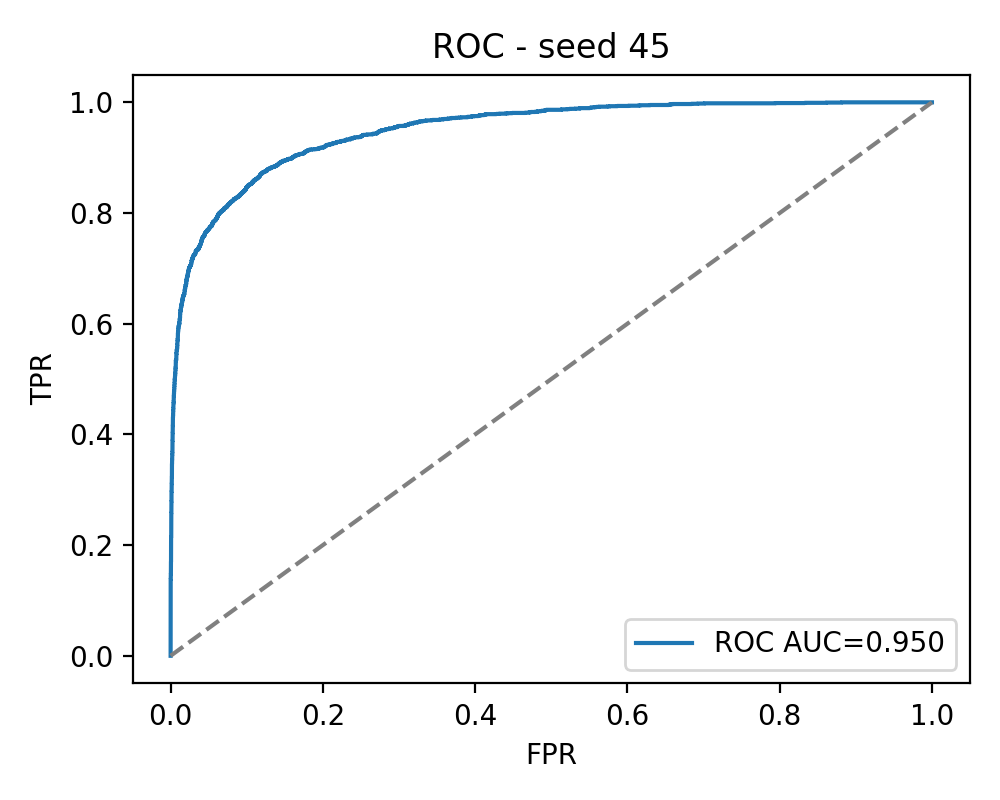
\includegraphics[width=.45\linewidth]{ablation_study/reports/grampa_split70-15-15_seed5_YYYYMMDD/figures/seed_42/roc.png}
  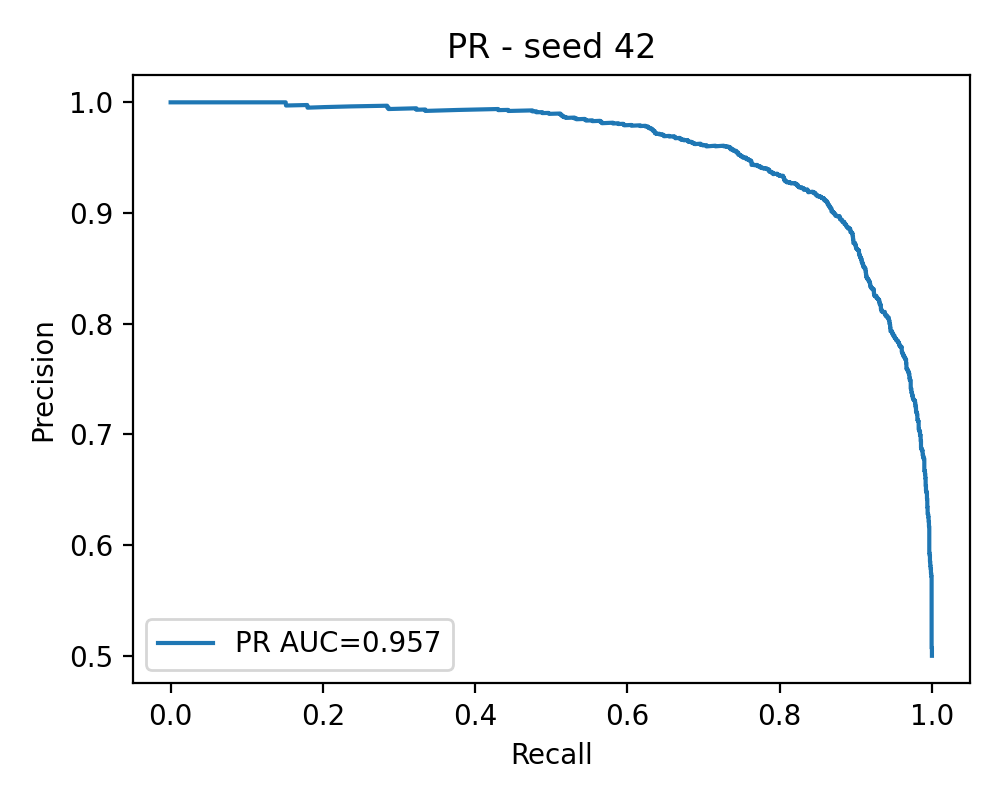
\includegraphics[width=.45\linewidth]{ablation_study/reports/grampa_split70-15-15_seed5_YYYYMMDD/figures/seed_42/pr.png}
  \caption{ROC and PR curves for a representative seed.}
\end{figure}

\begin{figure}[h]
  \centering
  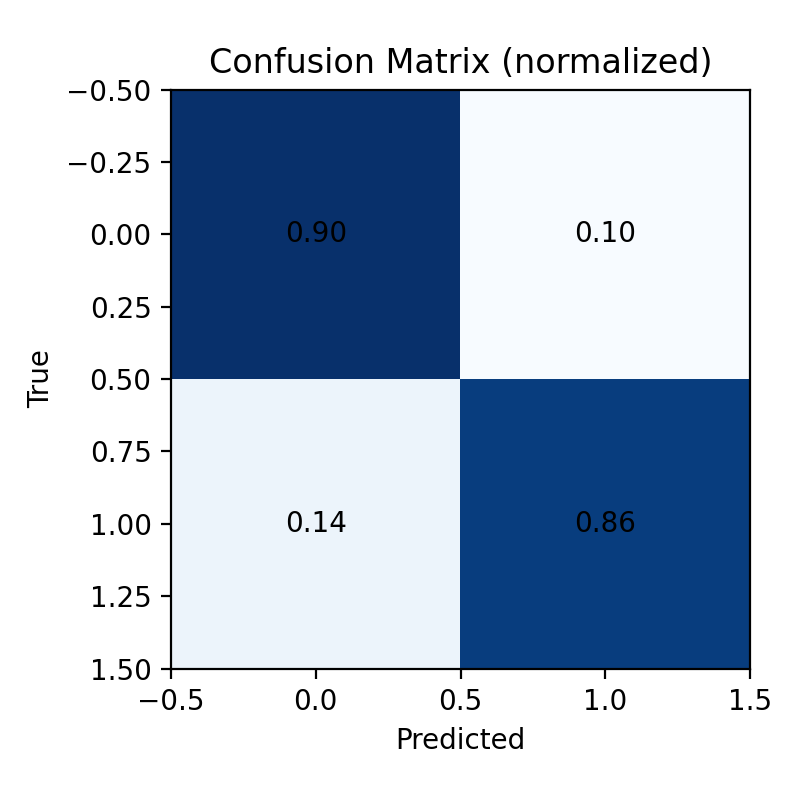
\includegraphics[width=.45\linewidth]{ablation_study/reports/grampa_split70-15-15_seed5_YYYYMMDD/figures/seed_42/confusion.png}
  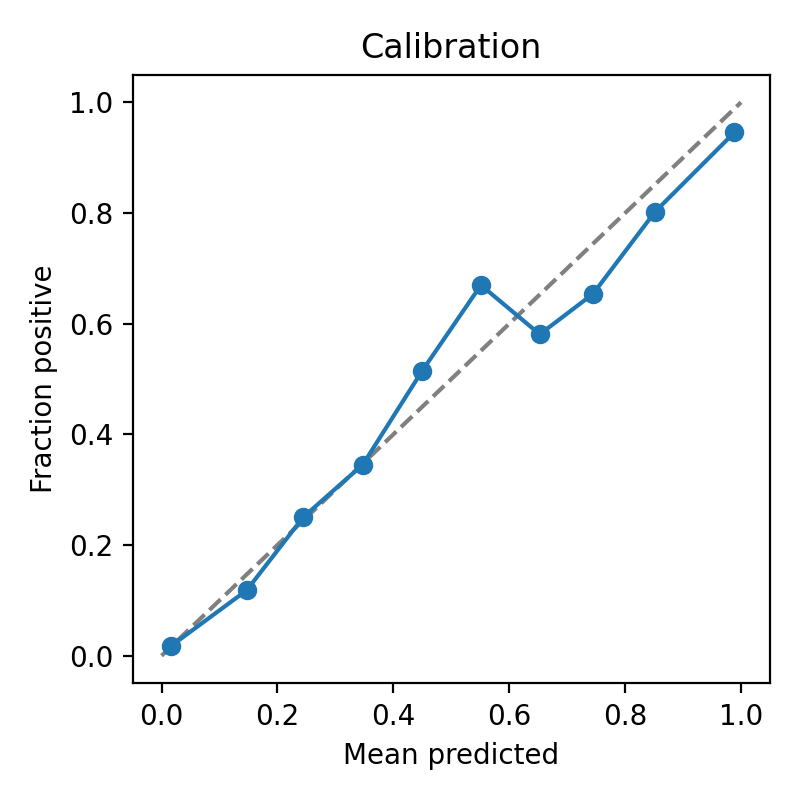
\includegraphics[width=.45\linewidth]{ablation_study/reports/grampa_split70-15-15_seed5_YYYYMMDD/figures/seed_42/calibration.png}
  \caption{Confusion matrix (normalized) and calibration plot for a representative seed.}
\end{figure}

\noindent \textbf{Aggregate}: The JSON summary at \texttt{.../tables/summary.json} contains \texttt{accuracy\_mean}, \texttt{accuracy\_std}, \texttt{auc\_mean}, \texttt{auc\_std}. These constitute the headline numbers for the report.

\section{Discussion}
\begin{itemize}[leftmargin=*,nosep]
  \item \textbf{Strengths}: End\-to\-end automation; clear, reproducible evaluation; artifacts versioned; actionable diagnostics.
  \item \textbf{Limitations}: Data quality and label curation; potential leakage risks without grouped splits; DNA context as short segments rather than mechanistic targets.
  \item \textbf{Expectations vs. reality}: Claude accelerates boilerplate generation but needs careful data/validity checks; human curation remains essential.
\end{itemize}

\section{Next Steps}
\begin{itemize}[leftmargin=*,nosep]
  \item Peptide\-only vs dual\-input ablations; organism\-aware external tests (e.g., standardized MIC from DRAMP/DBAASP).
  \item Improved features (learned embeddings/transformers), class balancing, and probability calibration.
  \item Bridge back to PRM/multimodal evaluation (e.g., compare model recommendations under language\-guided constraints).
\end{itemize}

\section{Conclusion}
We built a functional dataset and dual\-branch predictor, established a robust 70/15/15 multi\-seed evaluation, and generated comprehensive figures and artifacts. This provides a solid foundation for continued research and extensions.

\section*{References}
Relevant datasets and literature (to be expanded): DRAMP, DBAASP; DreamPRM; peptide--bacteria activity studies.

\end{document}
